\begin{enumerate}[label=\alph*)]
    \item
        不是凸集, 理由如下:

        \begin{figure}[ht]
            \centering

            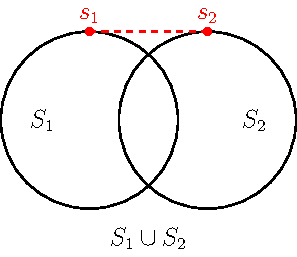
\includegraphics{figures/1a.pdf}
            \caption{}
            \label{figure:1a}
        \end{figure}

        如\cref{figure:1a}所示, 取图中$s_1\in S_1$, $s_2\in S_2$两点, $\lambda s_1+(1-\lambda)s_2$为图中红色虚线段.
        由于该线段不在$S_1\cup S_2$内, 因此$S_1\cup S_2$不是凸集.

    \item
        是凸集, 理由如下:

        $\forall s_1,s_2\in S_1+S_2$, s.t.
        \begin{equation*}
            s_1=x_1+y_1,\quad
            s_2=x_2+y_2,\quad
            x_1,x_2\in S_1,\quad
            y_1,y_2\in S_2.
        \end{equation*}

        $\forall\lambda\in[0,1]$, s.t.
        \begin{align*}
            \lambda s_1+(1-\lambda)s_2
            &=\lambda(x_1+y_1)+(1-\lambda)(x_2+y_2) \\
            &=[\lambda x_1+(1-\lambda)x_2]+[\lambda y_1+(1-\lambda)y_2],
        \end{align*}
        由于$S_1,S_2$均为凸集, 因此$\lambda x_1+(1-\lambda)x_2\in S_1$, $\lambda y_1+(1-\lambda)y_2\in S_2$,则
        \begin{equation*}
            \lambda s_1+(1-\lambda)s_2 \in S_1+S_2,
        \end{equation*}
        因此$S_1+S_2$是凸集.

    \item
        是凸集, 理由如下:

        $\forall s_1,s_2\in S_1-S_2$, s.t.
        \begin{equation*}
            s_1=x_1-y_1,\quad
            s_2=x_2-y_2,\quad
            x_1,x_2\in S_1,\quad
            y_1,y_2\in S_2.
        \end{equation*}

        $\forall\lambda\in[0,1]$, s.t.
        \begin{align*}
            \lambda s_1+(1-\lambda)s_2
            &=\lambda(x_1-y_1)+(1-\lambda)(x_2-y_2) \\
            &=[\lambda x_1+(1-\lambda)x_2]-[\lambda y_1+(1-\lambda)y_2],
        \end{align*}
        由于$S_1,S_2$均为凸集, 因此$\lambda x_1+(1-\lambda)x_2\in S_1$, $\lambda y_1+(1-\lambda)y_2\in S_2$,则
        \begin{equation*}
            \lambda s_1+(1-\lambda)s_2 \in S_1-S_2,
        \end{equation*}
        因此$S_1-S_2$是凸集.
\end{enumerate}
